\documentclass{article}
\usepackage[utf8]{inputenc}

\usepackage{xcolor}
\definecolor{GruvWhite}{HTML}{FBF1C7}
\usepackage{minted}
\usemintedstyle{tango}
\usepackage{graphicx}
\graphicspath{ {./} }

\title{Trabalho Prático de Matemática Discreta: Análise de Algoritmos de Ordenação}

\begin{document}

\maketitle

\begin{center}
\begin{tabular} {c c}
  \hline
  Membro 1 & Guilherme Martins Machado \\ [1ex]
  \hline
  Membro 2 & Lucas Pascoal \\ [1ex]
  \hline
  Membro 3 & Nome \\ [1ex]
  \hline
\end{tabular}
\end{center}

\section{Descrição e Análise do Algoritmo 1}

Nosso pseudocódigo para ordenação por inserção é apresentado como um procedimento denominado \textit{Insertion Sort}, que toma como parâmetro um arranjo \texttt{A[1..n]} contendo uma sequência de comprimento \texttt{n} que deverá ser ordenada. (No código, o número \texttt{n} de elementos em \texttt{A} é denotado por A⋅comprimento.) O algoritmo ordena os números da entrada no lugar: reorganiza os números dentro do arranjo A, com no máximo um número constante deles armazenado fora do arranjo em qualquer instante. O arranjo de entrada A conterá a sequência de saída ordenada quando Insertion-Sort terminar.

\begin{minted}[
framesep=2mm,
baselinestretch=1.2,
bgcolor=GruvWhite,
fontsize=\footnotesize,
linenos
]{text}
INSERTION-SORT(A)
    for j = 2 to A.comprimento
        chave = A[j]
        // Inserir A[j] na sequencia ordenada A[1..j-1]
        i = j - 1
        while i > 0 and A[i] > chave
            A[i+1] = A[i]
            i = i - 1
        A[i+1] = chave
\end{minted}

Esse algoritmo funciona para \texttt{A = \{5, 2, 4, 6, 1, 3\}}. O índice \texttt{j} indica a ``carta atual'' que está sendo inserida na mão. No início de cada iteração do laço \texttt{for}, indexado por \texttt{j}, o subarranjo que consiste nos elementos \texttt{A[1..j − 1]} constitui a mão ordenada atualmente e o subconjunto remanescente \texttt{A[ j + 1..n]} corresponde à pilha de cartas que ainda está sobre a mesa. Na verdade, os elementos \texttt{A[1..j − 1]} são os que estavam originalmente nas posições 1 a \texttt{j − 1}, mas agora em sequência ordenada. Afirmamos essas propriedades de \texttt{A[1..j − 1]} formalmente como um de invariante de laço:

\section{Descrição e Análise do Algoritmo 2}

O algoritmo quicksort é um método de ordenação muito rápido e eficiente, inventado por C.A.R. Hoare em 1960,O Quicksort é o algoritmo mais eficiente na ordenação por comparação. Nele se escolhe um elemento chamado de pivô, a partir disto é organizada a lista para que todos os números anteriores a ele sejam menores que ele, e todos os números posteriores a ele sejam maiores que ele. Ao final desse processo o número pivô já está em sua posição final. Os dois grupos desordenados recursivamente sofreram o mesmo processo até que a lista esteja ordenada.

O quicksort, como a ordenação por intercalação, aplica o paradigma de divisão e conquista. Descrevemos a seguir, o processo de três etapas do método de divisão e conquista para ordenar um subarranjo típico \texttt{A[p..r]}. Divisão: Particionar (reorganizar) o arranjo \texttt{A[p..r]} em dois subarranjos (possivelmente vazios) \texttt{A[p..q − 1]} e \texttt{A[q + 1..r]} tais que, cada elemento de \texttt{A[p..q − 1]} é menor ou igual a \texttt{A[q]} que, por sua vez, é menor ou igual a cada elemento de \texttt{A[q + 1..r]}. Calcular o índice q como parte desse procedimento de particionamento. Conquista: Ordenar os dois subarranjos \texttt{A[p..q −1]} e \texttt{A[q + 1..r]} por chamadas recursivas a quicksort. Combinação: Como os subarranjos já estão ordenados, não é necessário nenhum trabalho para combiná-los: o arranjo \texttt{A[p..r]} inteiro agora está ordenado. O seguinte procedimento implementa o quicksort.

\begin{minted}[
framesep=2mm,
baselinestretch=1.2,
bgcolor=GruvWhite,
fontsize=\footnotesize,
linenos
]{text}
QUICK_SORT(A,p,r)
    if p<r
        q = PARTITION(A, p, r)
        QUICKSORT(A, p, q-1)
        QUICKSORT(A, q+1, r)
\end{minted}

Para ordenar um arranjo \texttt{A}, inteiro, a chamada inicial é \texttt{QUICKSORT(A, 1, A⋅comprimento)}.
O particionamento do arranjo \texttt{A} para o algoritmo é chamado procedimento \texttt{PARTITION}, que reorganiza o subarranjo \texttt{A[p..r]} no \texttt{lugar}.

\begin{minted}[
framesep=2mm,
baselinestretch=1.2,
bgcolor=GruvWhite,
fontsize=\footnotesize,
linenos
]{text}
PARTITION(A, p, r)
    x = A[r]
    i = p - 1
    for j = p to r - 1
        if A[j] <= x
            i = i + 1
            trocar A[i] por A[j]
    trocar A[i + 1] por A[r]
    return i + 1
\end{minted}

O codigo acima mostra o funcionamento da funcao PARTITION para um arranjo de \texttt{r - p} elementos. \texttt{PARTITION} sempre seleciona um elemento \texttt{x = A[r]} como um elemento pivô ao redor do qual particionar o subarranjo \texttt{A[p..r]}. À medida que é executado, o procedimento reparte o arranjo em quatro regiões (possivelmente vazias). No início de cada iteração do laço for nas linhas 3−6.

\section{Análise Assintótica}

Representação em Ozão ou Theta da complexidade do algoritmo 1 no melhor e pior caso em relação ao tempo de execução:
\begin{itemize}
  \item{Para o melhor caso:}
    \begin{equation}
        \sum_{i=1}^{n-1}1= n - 1 = O(n)
    \end{equation}
  \item{Para o pior caso:}
    \begin{equation}
        \sum_{i=1}^{n-1}i= \frac{(n-1)n}{2} = \frac{n^{2}}{2} - \frac{n}{2}= O(n^{2})
    \end{equation}
\end{itemize}

Representação em Ozão ou Theta da complexidade do algoritmo 2 no melhor e pior caso em relação ao tempo de execução:

Na divisão mais equitativa possível, PARTITION produz dois subproblemas, cada um de tamanho não maior que \frac{n}{2}, já que um é de tamanho $\frac{n}{2}$ e o outro é de tamanho $\frac{n}{2} − 1$. Nesse caso, a execução do quicksort é muito mais rápida. Então, a recorrência para o tempo de execução é
\begin{itemize}
  \item{Para o melhor caso:}
    \begin{equation}
       T(n) = 2T(\frac{n}{2}) + \theta (n)
      \end{equation}
\end{itemize}
onde toleramos o desleixo de ignorar o piso e o teto e de subtrair 1. Pelo caso 2 do teorema mestre, a solução dessa recorrência é \texttt{T(n) = Q(n lg n)}. Balanceando igualmente os dois lados da partição em todo nível da recursão, obtemos um algoritmo assintoticamente mais rápido.

Particionamento no pior caso \texttt{O} para o quicksort ocorre quando a rotina de particionamento produz um subproblema com \texttt{n − 1} elementos e um com \texttt{0} elementos. Vamos considerar que esse particionamento não balanceado surja em cada chamada recursiva. O particionamento custa o tempo \texttt{Q(n)}. Visto que a chamada recursiva para um arranjo de tamanho \texttt{0} apenas retorna, \texttt{T(0) = Q(1)} e a recorrência para o tempo de execução é
\begin{itemize}
  \item{Para o pior caso:}
    \begin{equation}
      T(n) = T(n-1) + T(0) + \theta (n) = T(n-1) + \theta (n)
    \end{equation}
\end{itemize}
Intuitivamente, se somarmos os custos incorridos em cada nível da recursão, obteremos uma série aritmética (equação \texttt{(A.2)}), cujo valor chega a \texttt{Q(n2)}. Na realidade, é simples usar o método de substituição para provar que a recorrência \texttt{T(n) = T(n − 1) + Q(n)} tem a solução \texttt{T(n) = Q(n2)}.  Assim, se o particionamento é maximamente não balanceado em todo nível recursivo do algoritmo, o tempo de execução é \texttt{Q(n2 )}. Portanto, o tempo de execução do pior caso do quicksort não é melhor que o da ordenação por inserção. Além disso, o tempo de execução \texttt{Q(n2)} ocorre quando o arranjo de entrada já está completamente ordenado — uma situação comum na qual a ordenação por inserção é executada no tempo \texttt{O(n)}.

\subsection{Debate a respeito de quais algoritmos são mais eficientes em diferentes cenários}
\textit{Insertion Sort} é um algoritmo simples e eficiente quando aplicado em pequenas listas. Neste algoritmo a lista é percorrida da esquerda para a direita. A medida que avança, deixa os elementos mais à esquerda ordenados.

\textit{Quick Sort} (em portugues, ``ordenação rápida'') tem tempo de execução do pior caso de \texttt{Q(n2)} para um arranjo de entrada de n números. Apesar desse tempo de execução lento para o pior caso, muitas vezes, o quicksort é a melhor opção prática para ordenação, devido à sua notável eficiência na média. Seu tempo de execução esperado é \texttt{Q(nlg n)}, e os fatores constantes ocultos na notação \texttt{Q(nlg n)} são bastante pequenos. Também apresenta a vantagem de ``ordenar no lugar'' e funciona bem até mesmo em ambientes de memória virtual


\section{Análise Experimental}

\subsection{Metodologia}

Os testes foram executados em um computador pesssoal com:
\begin{itemize}
  \item{16 GB de memória RAM, 2400 MHz}
  \item{CPU Ryzen 5600x}
\end{itemize}
Uma bateria de 100 chamadas a ambos algoritmos eh feita a cada teste, realizando uma media entre o tempo em microssegundos de todas as chamadas ao final do processo. Ao todo, 200 testes foram feitos para ambos os algoritmos, com arranjos de 2 a 200 elementos.

Os elementos sao constituidos unica e exclusivamente de numeros inteiros entre 0 e 1000; sao gerados aleatoriamente pela funcoes \texttt{rand()} e \texttt{srand()}, tendo como sua ``semente'' o tempo interno da maquina de testes.

Uma implementacao \textit{in house} de ambos os algoritmos escrita na linguagem de programacao \texttt{C} foi feita pelos pesquisadores para averiguar a facilidade de implementacao e performance.

\subsection{Implementacoes}

Como dito anteriormente, a ferramenta eh uma funcao timer simples, \texttt{get\_time()}, que tem como valor de retorno o tempo decorrrido desde o \textit{Epoch}. Para obter o resultado, o tempo no inicio (\texttt{start}) eh subtraido do tempo no final (\texttt{end}):

\begin{itemize}
  \item{\texttt{timer.c}}
\end{itemize}
\begin{minted}[
framesep=2mm,
baselinestretch=1.2,
bgcolor=GruvWhite,
fontsize=\footnotesize,
linenos
]{c}
#include <sys/time.h>
#include <sys/resource.h>

double get_time()
{
    struct timeval t;
    struct timezone tzp;
    gettimeofday(&t, &tzp);
    return t.tv_sec + t.tv_usec*1e-6;
}
\end{minted}

\begin{itemize}
  \item{\texttt{algo-bench.c}}
\end{itemize}
\begin{minted}[
framesep=2mm,
baselinestretch=1.2,
bgcolor=GruvWhite,
fontsize=\footnotesize,
linenos
]{c}
int start = get_time();
    for (int i = 0; i < runs; i++) {
        quick_sort(qs_arr, 0, size-1);
    }
    printf("Average runtime length was: %lf\nSorted array is:\n",
            (get_time() - start)*1e6 / runs
    );
\end{minted}

\subsection{Resultados}

Os resultados dos testes experimentais estaos \textit{plotados} no grafico a seguir:

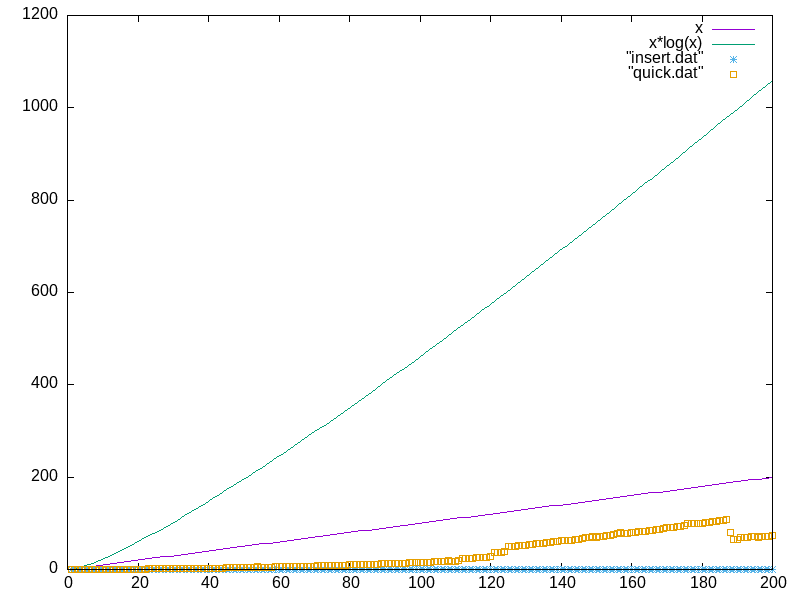
\includegraphics[scale=0.5]{graph}

Os resultados sao drasticamente contrastantes, como observado.

\section{Referências}

Referencias para a descricao do pseudo-codigo:

A funcao \texttt{PARTITION} se deve a N. Lomuto, \textit{Introduction to Algorithms}, 3rd edition Copyright © 2009 by The MIT Press.

Donald Knuth. \textit{The Art of Computer Programming}, Volume 3: Sorting and Searching, Third Edition. Addison-Wesley, 1997. ISBN 0-201-89685-0. Section 5.2.1: Sorting by Insertion, pp. 80–105.

Thomas H. Cormen, Charles E. Leiserson, Ronald L. Rivest, and Clifford Stein. \textit{Introduction to Algorithms}, Second Edition. MIT Press and McGraw-Hill, 2001. ISBN 0262032937. Section 2.1: Insertion sort, pp. 15–21.

Outras referencias

Lee, J., & Yeung, C. Y. (2018). \textit{Personalizing Lexical Simplification}. In Proceedings of the 27th International Conference on Computational Linguistics.

Mancini, P. (2011). \textit{Leader, president, person: Lexical ambiguities and interpretive implications}. European Journal of Communication, 26(1).

Saggion, H. (2018). \textit{LaSTUS/TALN at Complex Word Identification (CWI) 2018 Shared Task. In Proceedings of the Thirteenth Workshop on Innovative Use of NLP for Building Educational Applications}.

\end{document}
